\documentclass[letterpaper,10pt]{article}

\usepackage[english]{babel}
\usepackage[utf8]{inputenc}
\usepackage{amsmath}
\usepackage{graphicx}
\usepackage[top=0.75in, bottom=0.75in, left=0.9in, right=0.9in]{geometry}
%\usepackage[small]{titlesec}

\newcommand{\bes}{\begin{equation*}}
\newcommand{\ben}[1]{\begin{equation}\label{#1}}
\newcommand{\ees}{\end{equation*}}
\newcommand{\be}{\begin{equation}}
\newcommand{\ee}{\end{equation}}

%\titlespacing{\section}{0pt}{\parskip}{-\parskip}

\begin{document}

\begin{flushright}
{\Large CS598APK Project Report}
\end{flushright}
\vskip -0.1in
\hrule
\vskip 0.4in

\section*{Introduction}
This report is meant to be a companion to the in-class presentation which has already suitably covered an introduction and motivation; as such the report will jump in straight into a more in depth coverage of methodology and results. \vskip 0.1in

\section*{Methodology}
We would like to examine the error $\epsilon = |$Exact potential - QBX computed potential$|$ and it's dependence on $a$. Call $G(r) = \frac{1}{r}$, $f(r,a) = \frac{1}{\sqrt{r^2+a^2}}$, and the k-th order Taylor series expansion about $d$ and evaluated at $a=0$: 
$$T_k(r,d) = \sum^k_{n=0}\frac{(-d)^n}{n!}f^{(n)}(r,d)$$
So our error is: $$\epsilon = \int_\Omega G(r) \sigma(r) \, dr - \int_\Omega T(r,d) \sigma(r) \, dr$$ where $\sigma(r)$ is the density (vorticity in our physical example). We would like to reformulate this into a more obvious form without the integrals and the density factored out

Consider the action of the Fourier transform (FT) on the error:
$$\mathcal{F}[\epsilon] = \mathcal{F}\left[ \int G \, \sigma \, dr \right] - \mathcal{F}\left[ \int T \, \sigma \, dr \right]$$
and by the convolution theorem:
$$= \mathcal{F}[G] \, \mathcal{F}[\sigma] - \mathcal{F}[T]\,\mathcal{F}[\sigma] = \mathcal{F}[\sigma] \left(\mathcal{F}[G] - \mathcal{F}[T]\right)  $$
$$\mathcal{F}[T_k] = \sum_{n=0}^k \frac{(-d)^n}{n!} \mathcal{F}[f^{(n)}(r,d)]$$
This form presents a much more convenient form for the error, one now should examine $\mathcal{F}[G] - \mathcal{F}[T]$ with respect to $d$.

It is known that $\mathcal{F}[1/r] = 1/\pi k^2$
\subsection*{Fourier Transforms}
We would like to take the Fourier transform of $\frac{1}{\sqrt{r^2+a^2}}$. The FT was not found after surveying a number of FT tables, so it must be computed. Therefore one needs to take the 3D Fourier transform. Both $G$ and $T$ are radially symmetric, so a natural approach is to apply a change of coordinates from Cartesian to spherical coordinates. Additionally, since one is free to orient $\vec r$, orient it along the $z$-axis so that $\vec k \cdot \vec r = |k||r| \, cos\,\theta$. This yields:


\begin{align*}
\int_{-\infty}^\infty\int_{-\infty}^\infty\int_{-\infty}^\infty \frac{1}{\sqrt{r^2+a^2}}e^{-2 \pi i\vec k\cdot \vec r }\,dx\,dy\,dz&=
\int_0^\infty\int_0^\pi \int_0^{2\pi} \frac{e^{-2 \pi ikr\cos(\theta)}}{\sqrt{r^2+a^2}}\,r^2\,\sin(\theta)\,d\phi\,d\theta\,dr\\\\
&=2\pi \int_0^\infty \int_0^\pi \frac{e^{-2 \pi ikr\cos(\theta)}}{\sqrt{r^2+a^2}}\,r^2\,\sin(\theta)\,d\theta\,dr\\\\
&=2\pi \int_0^\infty \frac{r^2}{\sqrt{r^2+a^2}} \int_0^\pi  e^{-2 \pi ikr\cos(\theta)}\sin(\theta)\,d\theta\,dr\,\\\\
&=2\pi \int_0^\infty \frac{r^2}{\sqrt{r^2+a^2}}\left(\frac{\sin(2\pi kr)}{\pi k r}\right)\,dr
\end{align*}
We now find that the integral fails to converge, since $\frac{r}{\sqrt{r^2+a^2}} \to 1$ as $r \to \infty$, and so $\frac{r}{\sqrt{r^2+a^2}} \sin(2\pi kr)$ is undamped. However, we expect that a value for the integral exists since one exists for $\int_0^\infty sin(2 \pi kr) \,dr = 1/2 \pi k $, the ``physicist's point charge'' (indeed, one takes this same approach to find the FT of $1/r$ in 3D to get $\mathcal{F}[1/r] = 1/\pi k^2$). The approach take is to introduce a screening term $e^{-br}, b>0$ in the integral which artificially damps the integrand and forces it to converge, then take the limit as $b\rightarrow 0$. Applying the same principle here:

\begin{align*}
\frac{2}{k} \int_0^\infty \frac{r}{\sqrt{r^2+a^2}}\,\sin(2\pi kr)\,dr &= \lim_{b \to 0}\, \frac{2}{k} \int_0^\infty \frac{r}{\sqrt{r^2+a^2}}\,e^{-b r}\sin(2\pi kr)\,dr\\\\
&= \lim_{b \to 0}\, \frac{2}{k} \int_0^\infty \frac{r}{\sqrt{r^2+a^2}}\, \frac{( e^{(b - 2 \pi k i)r} - e^{-(b + 2 \pi k i)r})}{2 i}\, dr\\\\
&= \frac{2}{\pi k^2} + \frac{i \pi a}{2k} (Y_1(-i 2 \pi a k)-Y_1(i 2 \pi a k))\\\\
&= \frac{2}{\pi k^2} - \frac{\pi a}{k} \operatorname{Im}Y_1(i 2 \pi a k)
\end{align*}

Where $Y_1$ is the Bessel function of the second kind and we have made us of it's definition to compute the integrand (and is readily verified in Mathematica).
If one computes in Mathematica the limit $\lim_{a \to 0} a Y_1(i 2 \pi a k) = i/\pi^2 k$, the limit of the Fourier transform for $a \to 0$ is simply $1/\pi k^2$, and we recover the Fourier transform of $1/r$ (i.e $1/\sqrt{r^2 + a^2}$ for $a=0$).

\subsection*{An alternate approach to the FT}
While the previous solution seems to reduce to the expected case for $a=0$, Mathematica and Fourier transform tables are unable to verify that the inverse Fourier transform recovers $1/\sqrt{r^2 + a^2}$. However, an alternate approach can be taken to deal with the lack of formal convergence of the integrand.

One could try to integrate by parts to arrive at an integrand that is better behaved, with the troublesome term being $\frac{r}{\sqrt{r^2+a^2}}$.

$$
u = \frac{r}{\sqrt{r^2+a^2}} \;\; u' = \frac{a^2}{(r^2+a^2)^{3/2}}\\\\
$$
$$
v' = \sin{2 \pi k r} \;\; v = \frac{- \cos{2 \pi k r}}{2 \pi k}
$$
$$
\int_0^\infty uv' \,dr = uv\Big|_0^\infty - \int_0^\infty u' v \,dr
$$
\begin{align*}
2\pi \int_0^\infty \frac{r^2}{\sqrt{r^2+a^2}}\left(\frac{\sin(2\pi kr)}{\pi k r}\right)\,dr &= \frac{2}{k}\left( \int_0^\infty \frac{a^2}{(r^2+a^2)^{3/2}}\, \frac{\cos{2 \pi k r}}{2 \pi k}\,dr - 
\frac{r}{\sqrt{r^2+a^2}} \, \frac{ \cos{2 \pi k r}}{2 \pi k} \Big|_0^\infty \right) \\\\
&=\frac{2}{k} \left( a K_1(2 \pi a k) - \lim_{r \to \infty}\left( \frac{r}{\sqrt{r^2+a^2}} \frac{\cos{2 \pi k r}}{2 \pi k} \right) \right) 
\end{align*}

Where $K_1$ is the Bessel function of the second kind and we have made us of it's definition to compute the integrand (and is readily verified in Mathematica).
The issue is the $\lim_{r \to \infty}\left( \frac{r}{\sqrt{r^2+a^2}} \cos{2 \pi k r}\right)$ which is in $[-1,1]$, but is otherwise unspecified. However, the limit  in $r \to \infty$ should be a value such that the resulting transform reduces to $1/\pi k^2$ when $a \to 0$, recovering the transform of $1/r$. By taking the limit in Mathematica of $\lim_{a \to 0} a K_1(2 \pi a k)$ yields $1/2 \pi k$, then we can see that $\lim_{r \to \infty}\left( \frac{r}{\sqrt{r^2+a^2}} \cos{2 \pi k r}\right)$ must be 0 for the transform to recover the desired behavior for $a \to 0$.

Indeed, if we now test the proposed transform by taking the inverse Fourier transform (using Mathematica to carry out the integral), we find:
$$
2\pi \int_0^\infty \frac{2a}{k} K_1(2 \pi a k) \left(\frac{\sin(2\pi kr)}{\pi k r}\right)\,dk = \frac{1}{\sqrt{r^2+a^2}}\\\\
$$

\subsection*{Fourier transform of Taylor expansion}
Now that we have a way of taking the FT of our modified kernel, we can get to the task of actually taking the FT of it's Taylor expansion. Thankfully we find that derivatives of $\frac{1}{\sqrt{r^2+a^2}}$ are actually damped with respect to $r$ (and so the integrand in the FT of all subsequent terms formally converges) so no manual intervention is necesarry when computing the FT in Mathematica.

A series of script functions were set up to automate the task of taking the FT of each term. One finds that the FT of higher order terms results in modified Bessel of the first kind with higher orders and higher powers of $k$ and $d$ (the parameter chosen to represent the expansion center distance). It is possible to find a general expression for the resultant Fourier transforms which has the form:
$$\mathcal{F}[T_k] = \sum_{n=-1}^k C_n \, d^{n+2} \, k^nK_n(2 \pi k d)$$
where the coefficients $C_n$ are dependant on the particular order of the Taylor expansion $k$ (not to be confused with the Fourier variable $k$). Note that this expression makes use of the fact that $K_{-1}(x) = K_1(x)$.

\section*{Results}
Now that closed form expressions have been obtained for the FT of any order expansion, let us examine their behavior. Figure 1 shows how well the expansion approximate the true kernel in Fourier space. While they do reasonably well qualitatively one issue is that the modified Bessel function of second kind have log(k)-type singularities at 0, while $G$ has a $k^{-2}$ singularity.

Figure 2 shows the k dependence of the error, which tells us how well the expansion preserves low vs high modes in real space. We can see that for 3rd order expansions and above the error for any one mode is bounded.

\begin{figure}
\centering
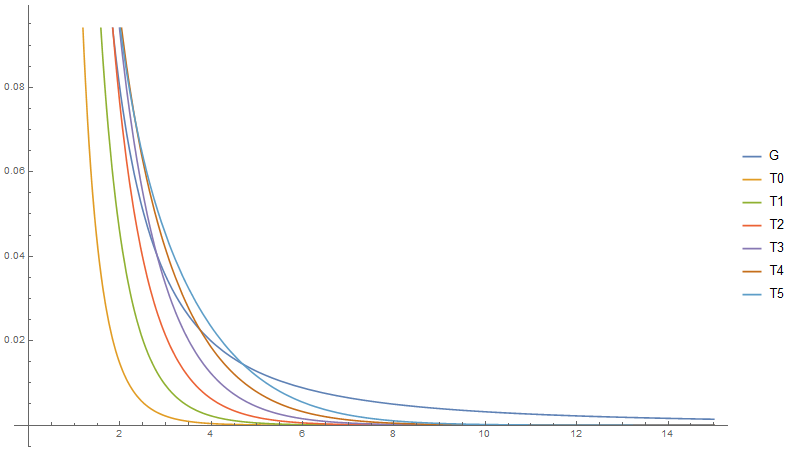
\includegraphics[width=5in]{T.PNG}
\caption{Behavior of expansions of modified kernel vs true kernel with respect to $k$, $d=0.2$}
\end{figure}

\begin{figure}
\centering
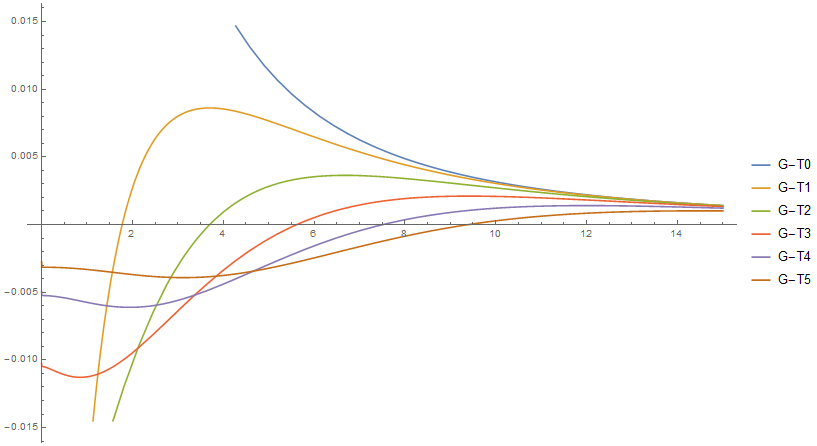
\includegraphics[width=5in]{G-T.PNG}
\caption{Behavior of error for expansions of modified kernel with respect to $k$, $d=0.2$}
\end{figure}

One way of thinking about the error quantitatively would be to examine $\int (\mathcal{F}[G]-\mathcal{F}[T])^2 \, dk$, we would like to minimize this. While $|\mathcal{F}[G]-\mathcal{F}[T]|$ is messy, as it turns out $\int (\mathcal{F}[G]-\mathcal{F}[T])^2 \, dk$ reduces concisely.
$$\int (\mathcal{F}[G]-\mathcal{F}[T_k])^2 = T_3: \frac{3 \pi ^3 d^3}{256}, T_4:\frac{175 \pi ^3 d^3}{32768} ,T_5: \frac{3059 \pi ^3 d^3}{1048576}$$
We pick up extra power of $d$ due to integration across all $k$ compared to at a particular $k$. A more fair error estimate would look at the inf-norm (i.e. the mode with the highest error, which will dominate convergence behavior in real space), where one would expect to recover the observed 2nd order behavior.

Alternately, consider the Taylor series expansion of $T_5$  in Fourier space with respect to $d$:
$$ \frac{1}{\pi k^2} +\frac{\pi d^2}{10}+ \frac{1}{20} \pi ^3 d^4 k^2+ \mathcal{O}(d^6)$$
We can see that the first term is precisely the FT of the unmodified kernel, but there are additional terms that would therefore appear in the error. The lowest order term is second order. In fact, if one examines the Taylor expansion in Fourier space for even higher order expansions one finds that they still retain that the lowest order term is second order. This therefore explains the empirically observed limitation of 2nd order convergence of the scheme.

\section*{Conclusion}
An error estimate was found that properly explains the observed 2nd order convergence of a QBX-like approach to evaluating volume potentials. It was found that examining the error in Fourier space provided an easier and more clear behavior of the error in the Taylor expansion of a modified kenrel compared to the original true kernel. After computing the various Fourier transforms a closed form expression was found for both the FT of the Taylor expansion, as well as the error. Both of these expressions showed that indeed the error convergence is restricted to second order.

These facts suggest the need for an alternate basis in Fourier space that is more able to represent the $k^{-2}$ singularity. An alternate basis in turn would suggest an appropriate de-singularized kernel in real space. One major caveat of this modification is that it hinges on the fact that an inverse Fourier transform exists and the result is smooth enough.
\end{document}